\documentclass{beamer}
\usepackage{beamerthemeshadow}
\usepackage{graphics}
\begin{document}
\title{An Analogical study of Hyperledger Fabric and Ethereum}  
\author{A V Aswin}
\date{\today} 

\frame{\titlepage} 

\frame{\frametitle{Table of contents}\tableofcontents} 


\section{Introduction} 
\frame{\frametitle{Introduction} 
EA graph G is a minor of a graph H if G can be obtained from a
subgraph of H by contracting edges.
}
\subsection{Problem Definition}
\frame{ 
\begin{block}{Minor Containtment Problem}
The minor containment problem is to determine, given two input
graphs G and H, whether H (has a subgraph which) is a minor of G
\end{block}
}

\section{Ethereum} 
\frame{\frametitle{Ethereum}
\begin{itemize}
\item Open-source, public, blockchain-based distributed computing platform and operating system featuring smart contract functionality. \pause
\item Ethereum was proposed in late 2013 by Vitalik Buterin, a cryptocurrency researcher and programmer. \pause
\item Its own crypto currency - Ether  \pause
\item Ether can be transferred between accounts and used to compensate participant mining nodes for computations performed \pause
\item Latest Release - Homestead
\end{itemize} 
}



\subsection{Architecture}
\frame{\frametitle{Architecture}
\begin{itemize}
\item Ethereum Blockchain stores the data, code and also runs the code in the EVM (Ethereum Virtual Machine).
\end{itemize}
\centering
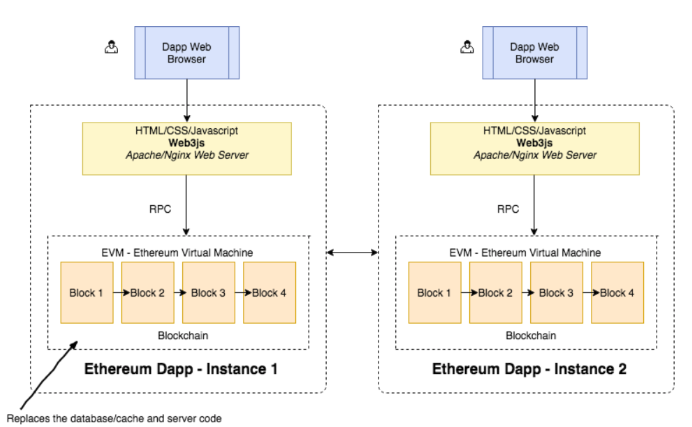
\includegraphics[height=4cm]{eth.png}
}

\frame{\frametitle{}
\begin{itemize}
\item All these computers (also called nodes) are connected to one another and have a full copy of the code and data.
\end{itemize}
\centering
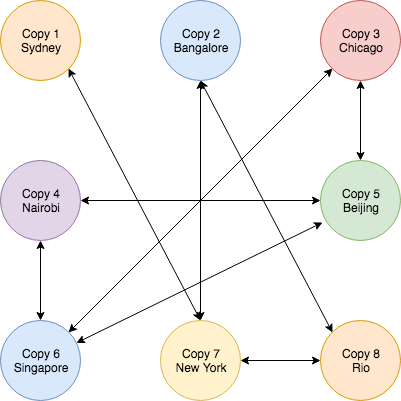
\includegraphics[height=4cm]{eth2.png}
}

\subsection{Addresses}
\frame{\frametitle{Addresses}
\begin{itemize}
\item In Ethereum blockchain, address is the identity. \pause
\item An Ethereum address looks like this: 001d3f1ef827552ae1114027bd3ecf1f086ba0f9 \pause
\item An address has a corresponding private key \pause
\item Pair of address+private key is needed to interact with the blockchain \pause
\item Ethereum address is public and the private key should never ever be shared with anyone
\end{itemize}
}

\subsection{Accounts}
\frame{\frametitle{Accounts}
\begin{itemize}
\item The combination of Ethereum address and it's private key is referred to as an account. \pause
\item An account in Ethereum can hold balance (Ether) and can send transactions \pause
\item Ethereum has 2 types of accounts. \pause
 \begin{enumerate}
     \item Externally owned accounts (EOA)
     \item Contract accounts
 \end{enumerate}
\end{itemize}
}

\frame{\frametitle{Gas, Gas Price and Gas Limit}
\begin{itemize}
\item There is a cost associated with each interaction with the ethereum blockchain. \pause
\item Need to pay Ether to the miners in the network to execute a transaction on the blockchain. \pause
\item Unit of work is called gas. \pause
\item Gas Price can be determined by the transaction initiator \pause
\item The higher the gas price set, the  transaction gets mined \pause
\item Gas limit which indicates the maximum amount of gas you are willing to buy to execute your transaction \pause
\item Block gas limit is the maximum cap applied to each block in Ethereum  \pause
\item Block can only include transactions whose total sum of gas is less than 8 million 
\end{itemize}
}

\subsection{Consensus Mechanism}
\frame{\frametitle{Consensus Mechanism}
\begin{itemize}
\item Currently, Ethereum uses mining based consensus algorithm called the Proof of Work. \pause
\item The proof of work algorithm used is called Ethash \pause

\centering
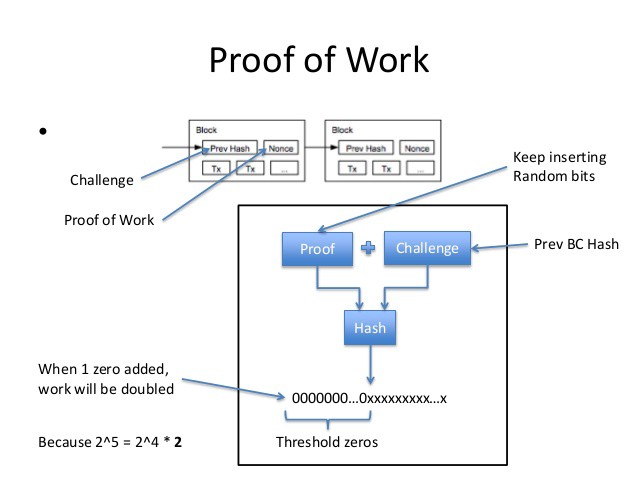
\includegraphics[height=4cm]{proof.jpeg} \pause
\item Ethash PoW is memory hard, making it ASIC resistant 

\end{itemize}
}

\subsection{dApps built on Ethereum}
\frame{\frametitle{dApps built on Ethereum}
\begin{itemize}
\item WeiFund - Decentralised Croudfunding platform. \pause
\item Airlock - Access protocol for smart property and Internet of Things \pause
\item Augur - Decentralised prediction market platform


\end{itemize}
}


\section{Hyperledger Fabric} 
\frame{\frametitle{Hyperledger Fabric}
\begin{itemize}
\item An open source enterprise-grade permissioned distributed ledger technology (DLT) platform \pause
\item Hyperledger was established under the Linux Foundation \pause
\item Fabric has a highly modular and configurable architecture \pause
\item Smart contracts authored in general-purpose programming languages such as Java, Go and Node.js
\end{itemize} 
}



\subsection{System Architecture}
\frame{\frametitle{System Architecture}

\centering
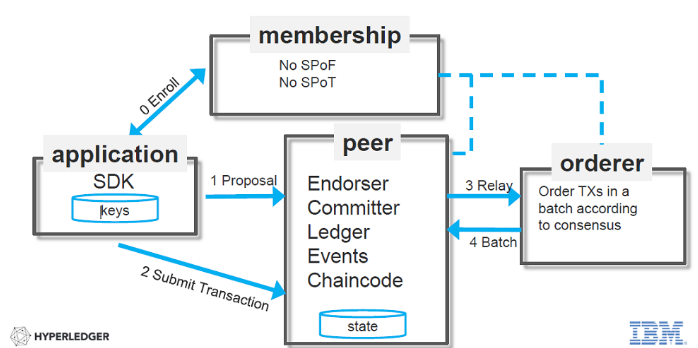
\includegraphics[height=4cm]{arch.png} \pause
}

\frame{\frametitle{Nodes}
There are three types of nodes :  \pause
\begin{itemize} 
\item Client or submitting-node  \pause
    \begin{itemize}
        \item The client represents the entity that acts on behalf of an end-user.
        \item  It must connect to a peer of its choice for communicating with the blockchain.
        \item Clients create and thereby invoke transactions.
    \end{itemize}
\item Ordering-service-node or orderer \pause
    \begin{itemize}
        \item provides delivery guarantees.
        \item provides a shared communication channel to clients and peers, offering a broadcast service for messages containing transactions.
        \item Clients create and thereby invoke transactions.
    \end{itemize}
\item Peers host ledgers and smart contracts.

\end{itemize}

}


\subsection{Workflow}
\frame{\frametitle{}
\centering
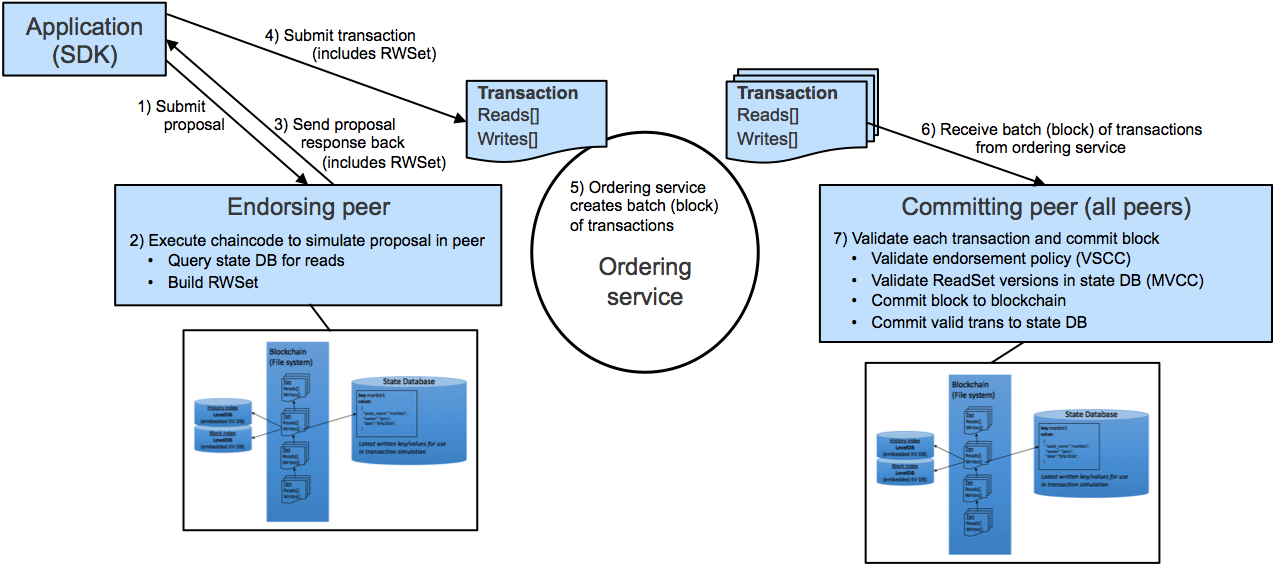
\includegraphics[height=4cm]{fabricarch.jpg}\pause
\begin{itemize}
\item The client creates a transaction and sends it to endorsing peers of its choice \pause
\item The endorsing peer simulates a transaction and produces an endorsement signature \pause
\item The submitting client collects an endorsement for a transaction and broadcasts it through ordering service \pause
\item The ordering service delivers a transactions to the peers 
\end{itemize}

}


\subsection{Ordering}
\frame{\frametitle{Ordering}
Hyperledger Fabric provides three ordering mechanisms: 
\begin{itemize}
\item SOLO : involves single ordering node \pause
\item Kafka : Kafka mechanism provides a crash fault-tolerant solution to ordering, based on Apache Kafka \pause
\item SBFT : Simplified Byzantine Fault Tolerance \\
             It can reach agreement even in the presence of malicious or faulty nodes

\end{itemize}
}

\section{Analysis} 
\subsection{Ethereum based Voting System}
\frame{\frametitle{Ethereum based Voting System }
\centering
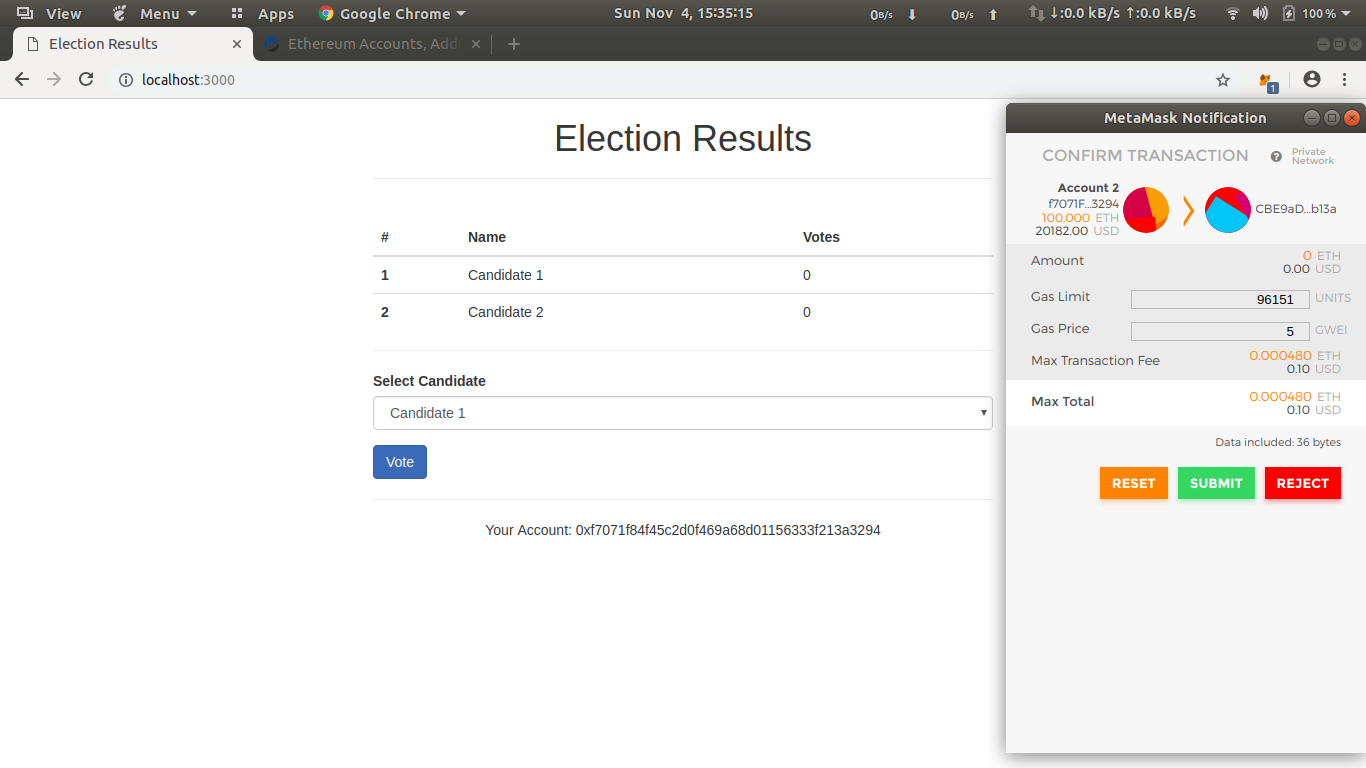
\includegraphics[height=4cm]{dapp1.png} 

}
\frame{\frametitle{ Ethereum Transaction Details }
\centering
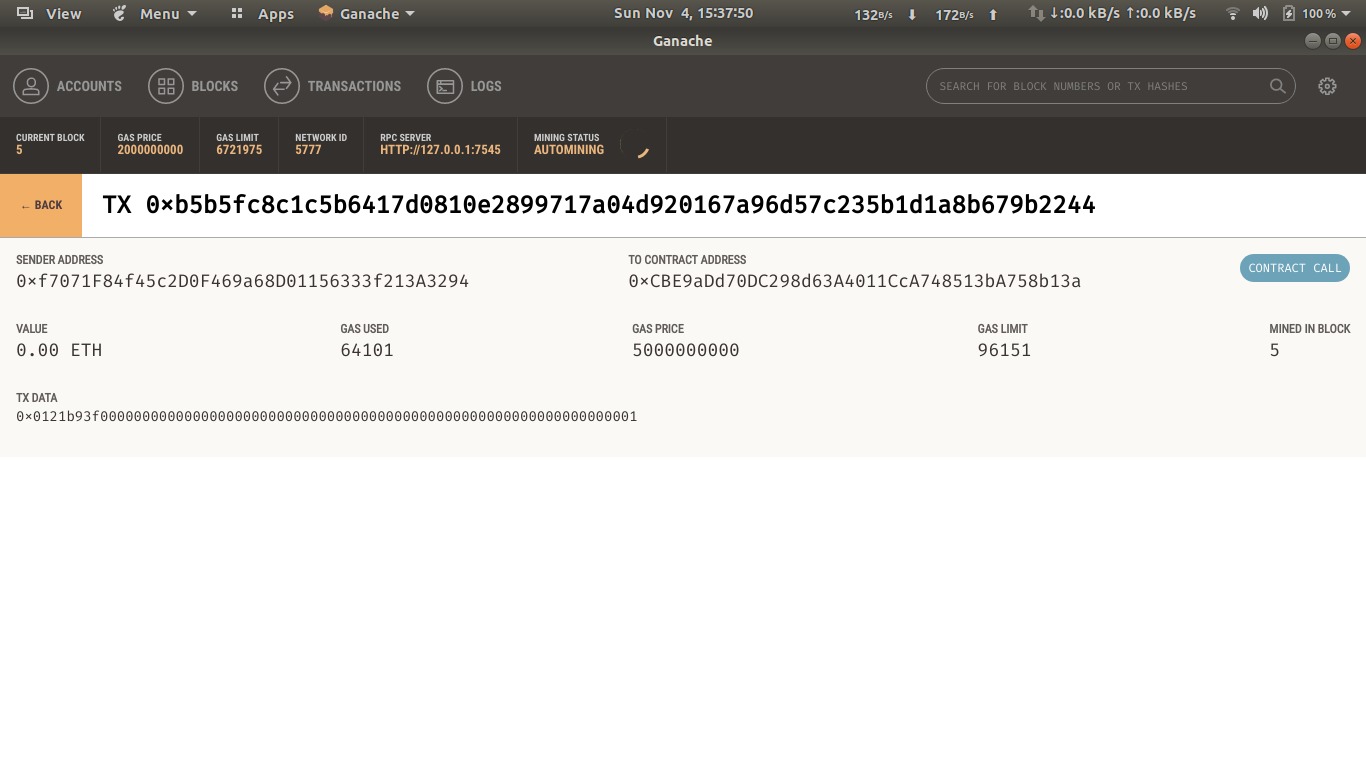
\includegraphics[height=4cm]{Transeth.png}

}
\frame{\frametitle{ Tools Used  }
\begin{itemize}
\item Truffle : development environment, testing framework and asset pipeline for Ethereum \pause
\item Ganache : personal blockchain for Ethereum development \pause
\item Metamask : bridge that allows us to visit the distributed web of tomorrow in your browser today.

\end{itemize}
}

\subsection{Fabric based Voting System}
\frame{\frametitle{Fabric based Voting System }
\centering
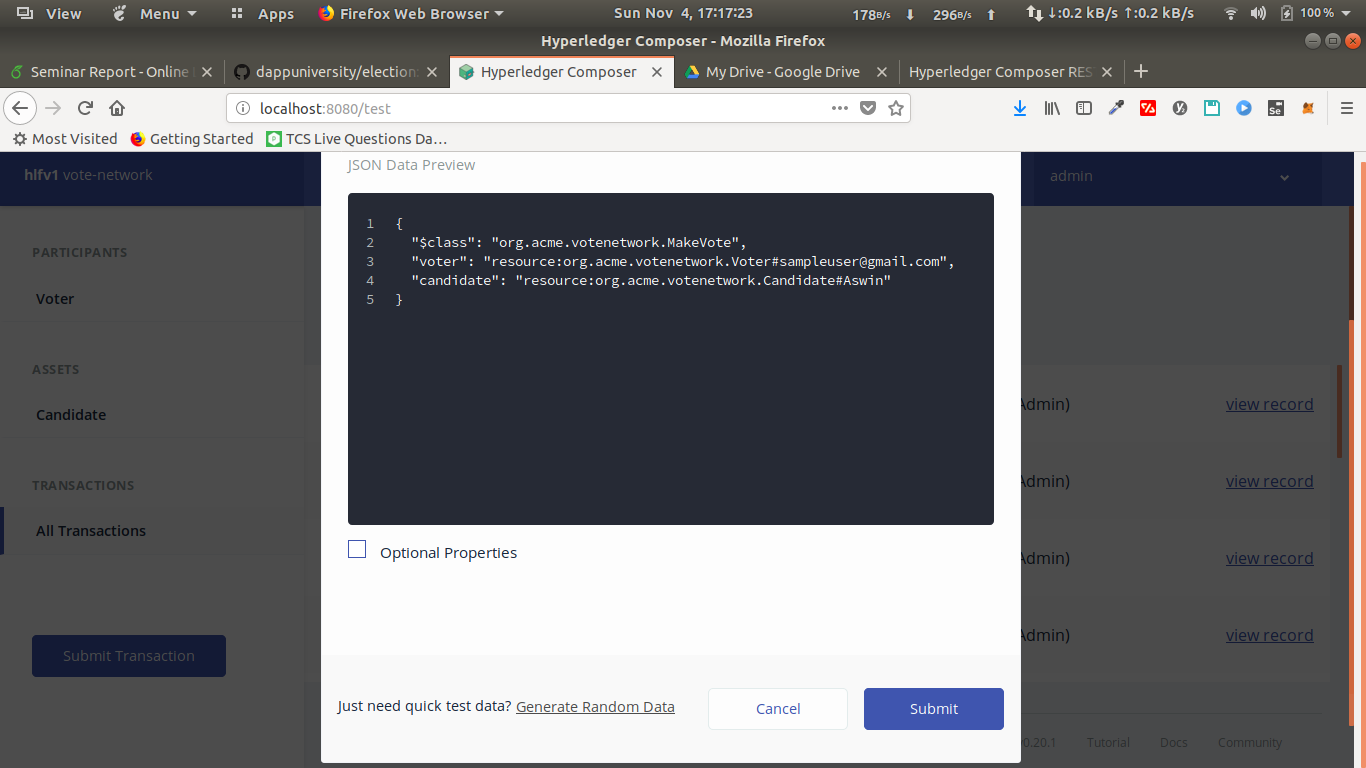
\includegraphics[height=4cm]{fabricapp.png}  

}
\frame{\frametitle{ Fabric Transaction Details }
\centering
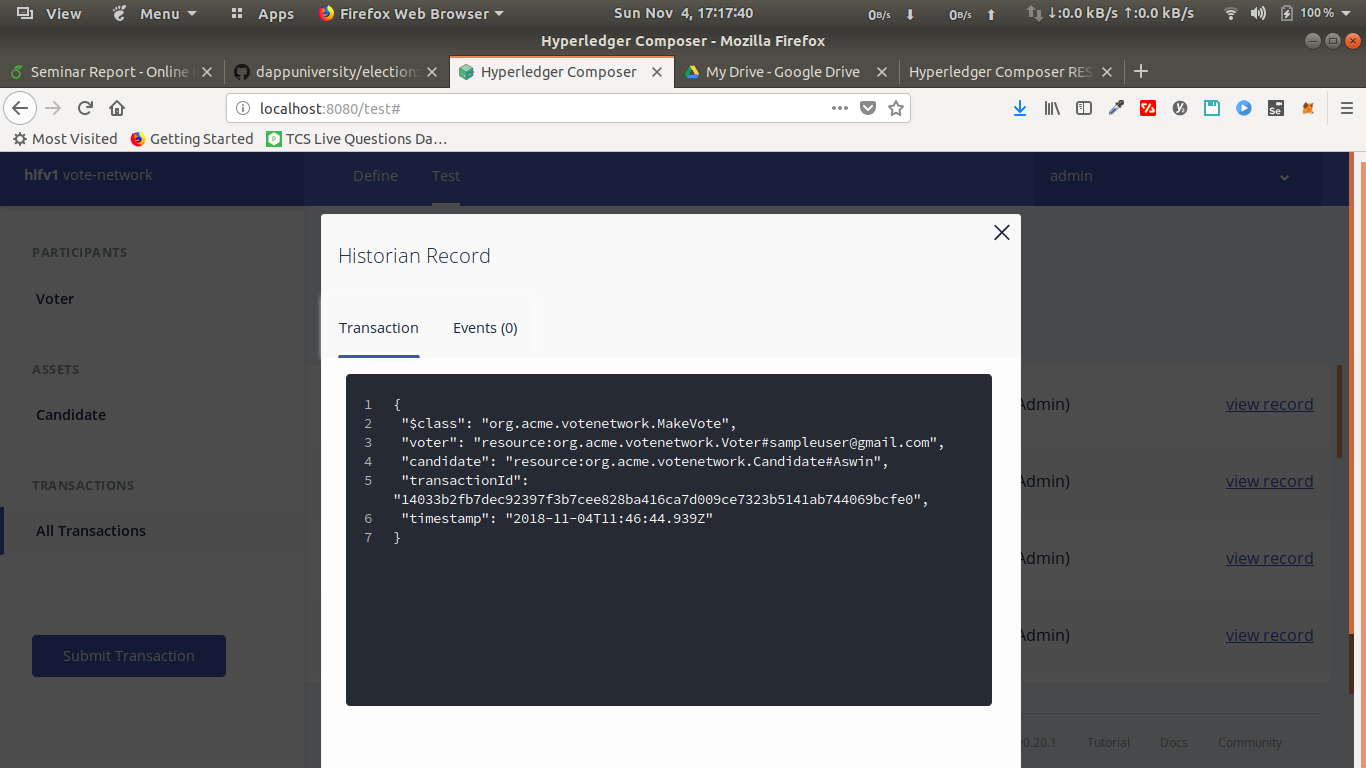
\includegraphics[height=4cm]{transfab.png}\pause

}

\frame{\frametitle{ Tools Used  }
\begin{itemize}
\item Composer Playground : provides a user interface for the configuration, deployment and testing of a business network \pause
\item Docker : tool designed to make it easier to create, deploy, and run applications by using containers \pause
\end{itemize}
}


\section{Comparison} 
\subsection{Performance}
\frame{\frametitle{Performance}
Analysis  in  the  paper  titled  ”Performance  Analysis  of  Private  BlockchainPlatforms in Varying Workloads”[4] shows that Hyperledger Fabric consistently performs better than Ethereum both in term of throughput and latency.
\begin{figure}
    \centering
    \begin{minipage}{0.45\textwidth}
        \centering
        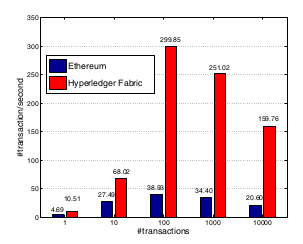
\includegraphics[width=0.9\textwidth]{throughput.png} 
        \caption{Average Throughput}
    \end{minipage}\hfill
    \begin{minipage}{0.45\textwidth}
        \centering
        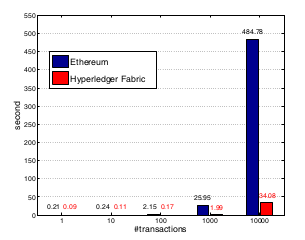
\includegraphics[width=0.9\textwidth]{latency.png} 
        \caption{Average latency}
    \end{minipage}
\end{figure}
}

\frame{\frametitle{SetPartitions algorithm}
\uncover<4->
{setPartions(n,k)\\}
\uncover<1-4>
{An intger array which stores the next partition\\}
\uncover<2-4>
{Initially set to {1,1,...1,2,3...,k}, the smallest lexicographic partition\\}
\uncover<3-4>{part[1..n]\\}
\uncover<4->{finished\\}
}

\frame{\frametitle{set partitions of S(5,3)}
\begin{center}
\begin{tabular}{|c|c|c|}
\hline
No & R(5,3) & S(5,3) \\ 
\hline
 1 & 11123 & 123.4.5 \\  
 2 & 11213 & 124.3.5 \\ 
 3 & 11223 & 12.34.5 \\
\hline
\end{tabular} 
\end{center}
}

\section{Bibliography} 
\frame{\frametitle{Reference}
\cite{Liu}
\cite{Graph}
\cite{wiki}
\bibliographystyle{alpha}
\bibliography{biblio}
}

\end{document}

